\chapter{Metoder til valg af model}
I det her kapitel vil vi redegøre for nogle metoder, således at vi kan finde den optimale model.
Vi er interesseret i en model der er god til at prædikterer, men uden at være for kompleks.  

For at prædikterer opdeles datasættet i et træningssæt med $t_0$ observationer og en testmængde med $T_0 = T - (t_0 +1)$ observationer, hvor $T$ er antallet af observationer af hele datasættet. 
Observationerne i træningsættet betragtes som in-sample observationer og anvendes primært til at identificerer modellen og estimere parametrene. 
Observationerne i testsættet betragtes som out-of sample observationer og fungerer som en referenceramme, når man vil vide hvor meget de prædikterede værdier afviger fra sande værdier 
 
\section{In-sample metoder}
I dette underafsnit vil vi introducerer metoderne, som er anvendt på vores træningsdata. Vi bruger træningsdata til at estimerer og identificerer vores model. 
Til at estimerer $\widehat{\lambda}$ i lasso modellen og generaliseringerne af lasso anvender vi to forskellige metoder nemlig krydsvalidering og BIC. 

\subsection{Krydsvalidering}
\textit{Denne sektion introducerer krydsvalidering, og er baseret på \citep{james} s. 175-184. }

Krydsvalidering er en metode, hvor vi estimerer prædiktions fejl fra træningssættet ved at holde fast i en del mængde. Delmængden bliver så anvendt som valideringssæt. 

Denne tilgang med at anvende et valideringssæt er en simple strategi for at estimerer prædiktions fejl på en mængde af observationer. 
Tilgangen splitter tilfældige observationer ind  i to delmængder, et træningssæt og et valideringssæt. 
Forskellige regressions modeller fittes på træningsdata og deres prædiktion af responsvariablen er evaluerede i valideringssættet. 
Valideringssættets fejl er normalt målt i MSE. 
Tilgangen med anvendelse af et valideringssæt er nem at implementere, men den har to ulemper. 
\begin{itemize}
\item Prædiktions fejlene kan være meget varierende, da fejlene afhænger af hvilken observationer der er inkluderet i træningssættet og valideringsættet. 
\item Idet denne tilgang deler vores data op i to delmængder vil vi derfor have færre observationer til at fitte vores model på. Derudover performere statistiske metoder sig dårligere på et træningsdata med færre informationer. Derfor kan valideringsættets have en tendens til at overestimere prædiktions fejlene for modellen, som er fitted på hele datasættet. ??
\end{itemize}
For at undgå disse to problemstillinger introduceres k-fold krydsvalidering. 

\subsubsection{k-fold krydsvalidering}
K-fold krydsvalidering deler observationerne ind i $k$ tilfældige grupper, hvor grupperne har  tilnærmelsesvis samme størrelse. 
Her anvender man den første gruppe, som valideringssættet og de resterende $k-1$ grupper, som træningssæt. 
Når metoden er fitted på de $k-1$ grupper udregnes MSE på de observationer i valideringssættet. 
Denne procedure gentages $k$ gange, og for hver gang anvendes en ny gruppe af observationer, som valideringssæt. 
Dette resulterer i $k$ estimater af prædiktions fejlene, $\text{MSE}_1, \text{MSE}_2, \dots , \text{MSE}_k $, hvor k-fold krydsvaliderings fejl er udregnet således
\begin{align}
\text{CV}_k = \frac{1}{k} \sum_{i=1}^k \text{MSE}_i \label{eq:cv_k}
\end{align}
Oftest er $k=5$ eller $k = 10$. 
Figur \ref{fig:cv_teori} illustrerer et 5-fold krydsvalidering. 
%
\begin{figure}
\center
\scalebox{0.7}{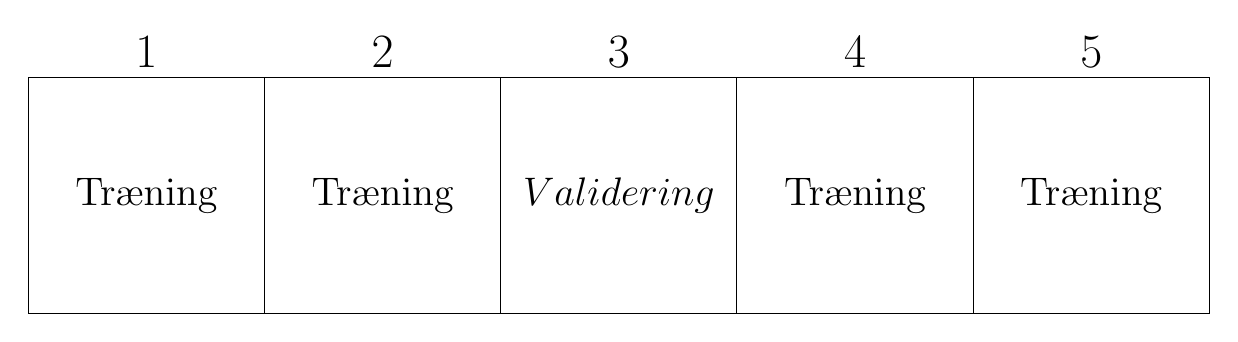
\begin{tikzpicture}
%\filldraw [green] (-3,0) circle (2pt) node [below, black]{$\widehat{\tmu}_0$};
\draw [-] (0,0) -- (15,0);
\draw [-] (0,3) -- (15,3);

\draw [-] (0,0) -- (0,3);
\draw [-] (15,0) -- (15,3);
\draw [-] (3,0) -- (3,3);
\draw [-] (6,0) -- (6,3);
\draw [-] (9,0) -- (9,3);
\draw [-] (12,0) -- (12,3);


\node[above] at (1.5,3) {\LARGE 1};
\node[above] at (4.5,3) {\LARGE2};
\node[above] at (7.5,3) {\LARGE3};
\node[above] at (10.5,3) {\LARGE4};
\node[above] at (13.5,3) {\LARGE5};

\node[align=left] at (1.5,1.5) {\Large Træning};
\node[align=left] at (4.5,1.5) {\Large Træning};
\node[align=left] at (7.5,1.5) {\Large $\text{Validering}$};
\node[align=left] at (10.5,1.5) {\Large Træning};
\node[align=left] at (13.5,1.5) {\Large Træning};

%\draw [<-] (1,4) node [above] {$\x_2$} --(-3,0);
%\draw [<-] (-5,4) node [above] {$\x_3$} --(-3,0);

\end{tikzpicture}}
\caption{5-fold krydsvalidering. I det her tilfælde fittes modellen i det første, andet, fjerde og femte gruppe af data og udregner prædiktions fejl af den fittede model for den tredje gruppe} \label{fig:cv_teori}
\end{figure} 
%
Et $k$-fold krydsvalidering har en lav varians, fordi ligning \eqref{eq:cv_k} tager det gennemsnitlige output af $k$ fittede modeller, som har en lav korrelation, siden vi har et relativt lille overlap mellem træningssættet i hver model. 
Bias kunne være et problem i forhold til hvordan vi vælger vores træningssæt. Hvis vi ikke har nok trænings observationer vil $k$-fold krydsvalidering have høj bias. Derfor er der også en bias-varians trade-off med valget af $k$. 

\subsection{BIC}
En anden tilgang til valg af turning parameteren $\lambda$ er ved anvendelse af BIC.
BIC bestemmes ud fra fittet og kompleksiteten af modellen. 
\begin{defn}[Bayesian informationskriterium (BIC)]\label{def:bic}
BIC er givet ved
\begin{align*}
\text{BIC} = \ln\del{t_0}p - 2 \ln\del{\widehat{L)}}, 
\end{align*}
hvor $\widehat{L}$ er den maksimerede værdi af likelihood funktion, $t_0$ er antallet observationer i træningssættet og $p$ er antallet af parameter.
\end{defn} 
Modellen med den laveste BIC vælges, da det indikerer, at modellen giver en god tilnærmelse af data i forhold til modellens kompleksitet. 
Hvis vi betagter en regressions model med normalfordelte residualer, så er maksimum likelihood estimatoren for variansen defineret som
\begin{align*}
\widehat{\sigma_p} = \frac{1}{t_0} \sum_{i=1}^{t_0} \del{y_i + \sum_{j=1}^p x_{ij}\beta_j}^2,
\end{align*}
Derfor har vi, at BIC 
\begin{align*}
\text{BIC} = \log \widehat{\sigma}^2_p + \frac{p \log t_0}{t_0},
\end{align*}
med samme notation som i definition  \ref{def:bic}.

\section{Out of sample metoder}
Målet med prædiktion er at prædiktere fremtidige værdier af en tidsrække. 
Vi prædikterer one step ahead med et expanding window. 
Det første window indeholder altså observationer fra tiden 1 til tid $t$, og den næste window indeholder observationer fra tiden 1 til $t+1$


%Den første rolling window indeholder altså observationer fra tiden 1 til $m$, og den næste rolling window indeholder observationer fra periode 2 til $m+1$ og sådan fortsætter det. 

Herpå måler vi prædiktions evnen via den gennemsnitlige kvadrede fejl (MSE). 
\begin{align}
\text{MSE} & =  \frac{1}{T_0} \sum_{t=t_0 +1 }^{T} \del{y_t - \widehat{y}_t}^2 
\end{align} 
hvor $T_0$ er antallet af observationer i testsættet, $y_t$ er observationen til tiden $t$ og $\widehat{y}_t$ er prædiktionen af $y_t$.
Funktionen vil have en værdi på 0, hvis et perfekt prædiktion, og ellers vil vi havde positive værdier. Så derfor er vi interesseret i den lavest værdi af MSE. 

En måde at vurdere to konkurrerende prædiktioner i forhold til hinanden er ved anvendelse af Diebold-Mariano testen. 
Vi lader $\widehat{y}_t^1$ og  $\widehat{y}_t^2$ være to konkurrerende prædiktioner af $y_t$, hvor $t = t_0 + 1, \dots, T$. 
De tilsvarende prædiktionsfejl er defineret ved $\epsilon^i_t = y_t - \widehat{y}^i_t $,  hvor $i = 1, 2$. 
Vi anvender en tabs funktion til at bestemme nøjagtigheden. Tabs funktionerne kan eksempelvis være $ L\del{\epsilon^i_t} = \del{\epsilon^i_t }^2 $ eller $L\del{\epsilon^i_t}  = \abs{\epsilon^i_t }$
%
Diebold Maraino testen er baseret på differensen af tabsfunktionerne
%
\begin{align*}
d_t = L\del{\epsilon^1_t} - L\del{\epsilon^2_t}
\end{align*}
%
%
\begin{defn}[Diebold-Mariano test (DM)]
Betragt $\hyp_0 : E[d_t] = 0$ imod  $\hyp_A : E[d_t] \neq 0$. 
Diebold-Mariano testen er defineret som følgende 
\begin{align*}
\text{DM} = \frac{\bar{d}}{\del{\widehat{\text{avar}}\del{\bar{d}}}^{\frac{1}{2}}} =  \frac{\bar{d}}{\del{\frac{\widehat{\text{LRV}}_{\bar{d}}}{n}}^{\frac{1}{2}}},
\end{align*}
hvor $\bar{d} = \frac{1}{T_0} \sum^{T}_{t = t_0 +1} d_t$ og $\text{LRV}_{\bar{d}} = \gamma_0 + 2\sum_{j = 1}^{\infty} \gamma_j$, hvor $\gamma_j = \Cov{d_t}{d_{t-j}}$. 
\end{defn}
%
Det kan vises, at teststørrelsen DM er asymptotisk standard normalfordelt under nulhypotesen. Derfor afvises nulhypotesen ved niveau $5 \%$, hvis $\abs{\text{DM}} > 1.96$
